
\chapter{引言}
\label{chap:introduction}

\section{研究背景}
近二十年来,计算机以及智能终端的计算和存储能力都得到了巨大的飞跃,互联网的信息量也呈现出爆炸式的增长。互联网的发展不仅为计算机技术带来许多新的问题和场景,同样给活在信息时代的人们提出了巨大的挑战。在每天生成的大量数据面前,如何高效的筛选出自己需要的信息成了大多人都需要面对的问题。据统计\citep{website:WWW},目前最主要的搜索引擎google每天新增的网页量高达40亿。

\begin{figure}[!htbp]
    \centering
    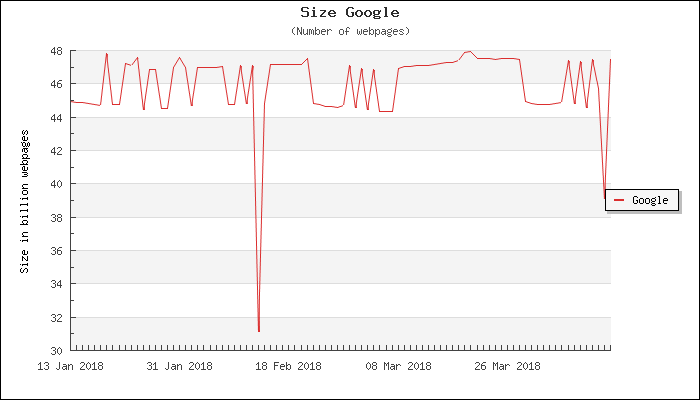
\includegraphics[width=0.80\textwidth]{google}
    \bicaption{google 2018年1-3月网页增长量}{The increment of web page indexed by google between 2018.1 to 2018.3}
    \label{fig:user-ad-match}
\end{figure}

数据量的增长不仅意味着高效的信息获取变得困难,同样意味着会有大量重复冗余的信息生成。如何去除冗余的信息,同样是一个巨大的问题。

文本长期以来一直都是人类信息传播的主要载体。人类大部分的知识都是以文本的形式进行记录和传播的,而人类自幼就开始学习如何从文本中获取信息,虽然互联网的发展大大促进了视频和语音的传递,但是文本仍然是大多数人获取信息的高效和主要手段。而文本匹配作为信息检索和冗余文本消除的基础,在各大互联网公司得到了广泛的使用。

\begin{figure}[!htbp]
    \centering
    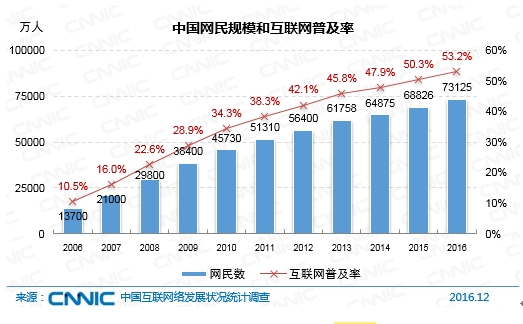
\includegraphics[width=0.80\textwidth]{CNNIC}
    \bicaption{中国网民和互联网普及率}{Chinese internet users and internet penetration rate}
    \label{fig:CNNIC}
\end{figure}

不仅如此,在自然语言处理中,需要任务如信息获取,问答系统,机器翻译,对话系统等等,都不同程度的需要用到文本匹配技术。根据使用场景的不同,文本匹配可以被分为三类:短文本-短文本匹配,短文本-长文本匹配以及长文本-长文本语义匹配。

1. 短文本-短文本匹配

短文本-短文本的匹配被广泛使用在工业界。如网页搜索中,搜索引擎必须计算用户的查询(query) 和网页标题(web page title)的语义相关性,并在此基础上结合用户画像进行排序返回给用户;在知乎,Quora等问答网站上需要进行相似问题的合并,这时我们需要度量一个问题和其他问题之间的相似度。这些场景都需要短文本-短文本的匹配作为基础。

\begin{figure}[!htbp]
    \centering
    
\includegraphics[width=1.0\textwidth]{ques_red}
    \bicaption{知乎问题重定向}{Question redirection in zhihu}
    \label{fig:ques_red}
\end{figure}

以相似问题的检测为例,对于两个给定的问题,我们用一个函数映射 $f:x\to \mathbb{R}^k$ 将句子中的每个词映射到一个高维的向量空间,得到句子的矩阵映射。在句子矩阵映射的基础上,我们可以选择利用深层网络建模单个句子的语义信息,或者直接利用深层网络建模句子之间的交互信息,最后将两个句子的语义信息或者句子的交互信息映射成一个一维的概率表达。

2. 短文本-长文本匹配

短文本-长文本语义匹配同样在在工业界被广泛运用,信息检索就是典型的短文本-长文本的匹配场景。这种场景中我们需要首先利用倒排索引等手段对网页正文建立索引,根据用户的输入利用事先建立的索引初步召回候选文档;然后利用文本匹配算法计算用户输入的查询和候选文档的相似度。在计算用户查询和网页正文的语义相关度时,由于用户查询通常较短,而网页正文较长,因此查询与正文的匹配与上文提到的短文本-短文本不同,通常需要使用短文本-长文本语义匹配,以得到更好的匹配效果。在计算相似度的时候,我们规避对短文本直接进行主题映射,而是根据长文本的主题分布,计算该分布生成短文本的概率,作为它们之间的相似度。
利用匹配算法计算出的相似度结合用户画像等排序得到最后的结果呈现给用户。

用于长文本相比于短文本的语义更加丰富,段落之间层次化的组织结构以及上下之间的语义关系使得短文本-长文本的匹配问题更加复杂。

3. 长文本-长文本匹配
由于长文本的语义丰富,上下文之间语义关系负责,因此长文本-长文本的匹配往往基于自动摘要或者主题模型等等方式,将长文本压缩到相同的高维空间,通过高维空间的距离衡量2个文本的相似度。高维空间的距离可以利用Hellinger Distance\citep{website:Hellinger}和Jensen-Shannon Divergence(JSD)\citep{website:Shannondivergence}。长文本-长文本的匹配往往用于新闻推荐等领域。

\begin{figure}[!htbp]
  \centering
  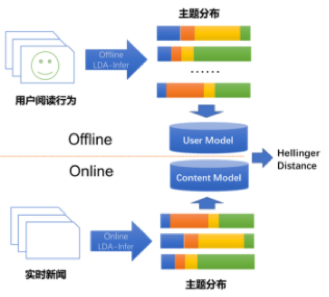
\includegraphics[width=0.6\linewidth]{news_com}
  \caption{新闻个性化推荐}{news recommendation}
  \label{fig:news_recom}
\end{figure}

\section{研究意义}
文本匹配是自然语言处理的重要问题,在信息检索、广告计算等领域有着广泛的应用,网页搜索,相似问题合并等等都需要文本匹配作为基础。早期的文本匹配算法往往是对词向量空间如VSM,BM25等的匹配,主要解决基于词汇层面的匹配问题。但是基于词汇层面的匹配只能解决词汇的相似,很难处理语义匹配;同时算法的泛化能力不足,在面对新任务时,必须重新设计特征和算法。

一个优秀的文本匹配算法必须要解决以下三个问题:

1. 语言多义性。相同的词语在不同语境下可能拥有不同的含义,如 “苹果” 既可以表示水果,也可以表示科技公司;而不同的词语也可以表达相同的语义,如 “出租车”,“的士”。

2. 语言的组合结构。由相同词语组成的句子由于语序的不同,也可能产生不同的语义。例如 “机器学习” 和 “学习机器”。

3. 匹配的非对称性问题。文本匹配任务并不一定要求语言相似,例如网页搜索中的查询和网页;也不一定要求语义上的相似,例如问答系统。

基于词汇的匹配模型显然无法解决这种问题。因此从上世纪 90 年代开始,有人开始尝试将主题模型应用于文本匹配,主题模型可以较好地表示文本的语义信息,从而弥补传统文本匹配算法的不足。但是从效果上看,他们都无法替代基于词汇的匹配方法,只能作为补充。
在世纪初,计算机的计算力和存储量开始爆炸式增长,因此开始有人尝试将深度学习应用于文本匹配算法上并且取得了较好的效果,
目前大部分的深度学习算法都试图利用神经网络理解语义信息,但是现阶段计算机仍然难以理解语义信息,因此基于语义信息的文本匹配算法目前具有天然劣势。

\begin{figure}[!htbp]
    \centering
    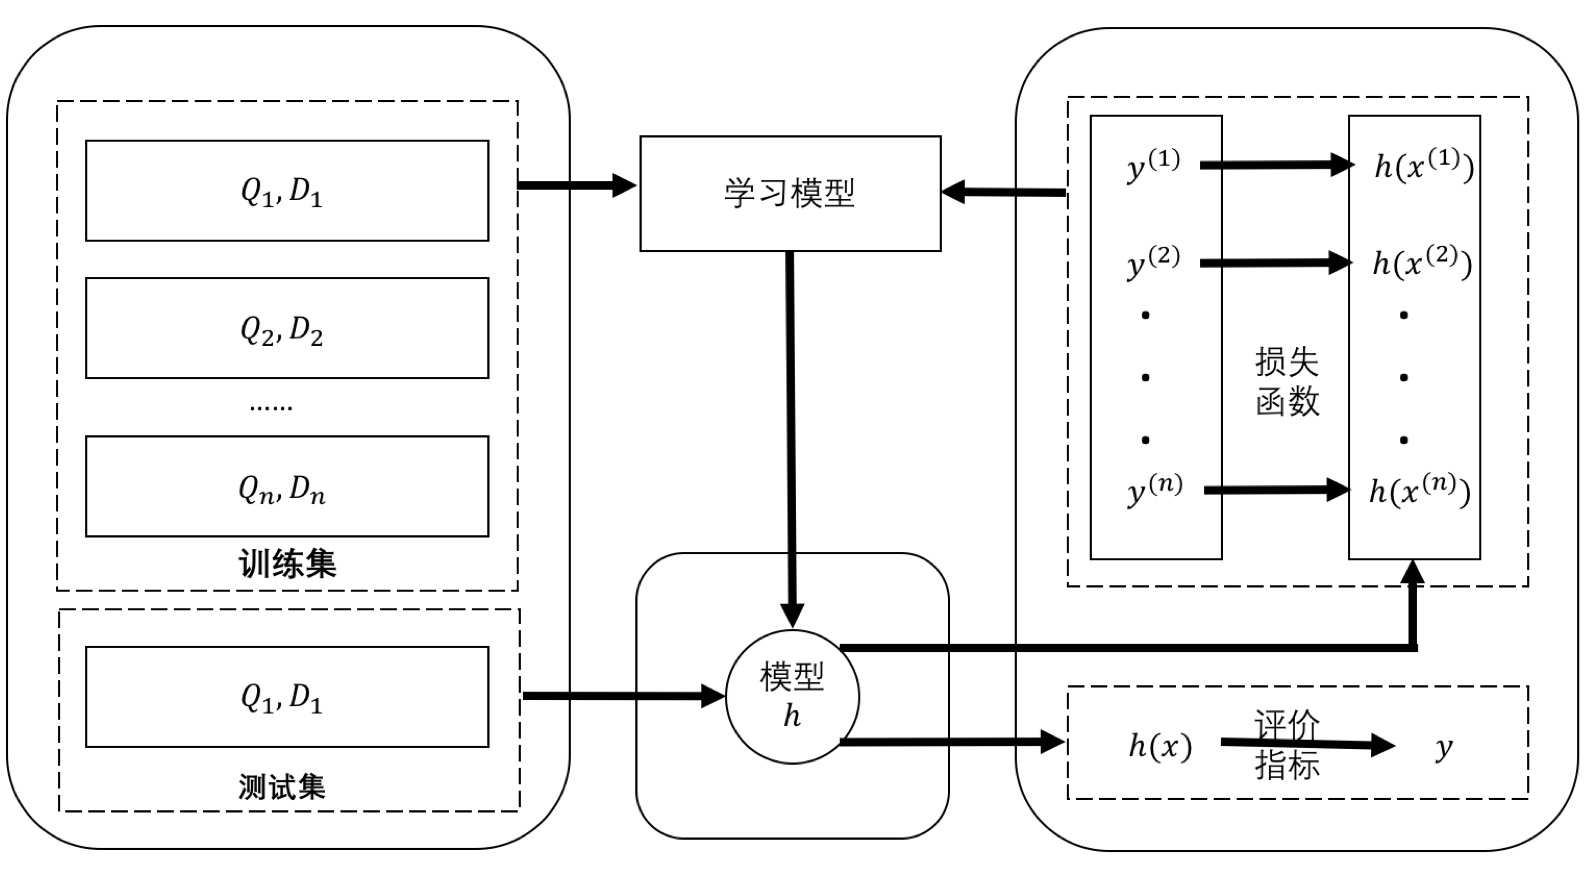
\includegraphics[width=1.0\textwidth]{match_learn_arch}
    \bicaption{文本匹配框架}{The architecture of text matching}
    \label{fig:match_learn_arch}
\end{figure}

文本匹配的算法框架如图 \ref{fig:match_learn_arch} 所示,概括了文本匹配算法中的三个主要部分:模型,数据集和评价指标。一般来说,文本匹配的数据集中正例样本为人工标注,负样本通过在整个句子空间中随机抽取句子对构成。

由于传统的模式匹配方案模式规则难以维护、系统复杂,因此近几年来对文本匹配的研究集中于深度学习,即利用深度网络学习到文本的语义信息进行匹配。但是计算机对语义理解的困难为语义匹配的方案引入了额外的复杂度,算法工程师必须进行巧妙的特征设计以应对不同的业务场景。

近几年来,深度网络极大的增强了强化学习表达能力,使得强化学习建模现实世界问题的能力越来越强。近年来,强化学习已经在游戏,围棋等等方面超越人类的表现。强化学习在规则学习方面表现出了强大的能力,部分场景下甚至可以在没有人类先验知识指导的情况下获得令人惊讶的学习能力。而文本匹配所存在的规则远远没有围棋等复杂,但是目前为止还没有人尝试利用强化学习进行文本匹配的研究,因此利用强化学习学习传统文本匹配中的规则拥有强大的潜力。

\section{本文贡献}
文本匹配是传统的自然语言处理问题,传统的基于模式匹配的方案往往规则复杂,系统难以维护;现在基于深度学习的语义匹配拥有天生的缺陷。而深度强化学习由于其强大的建模能力开始在各个场合发挥越来越重要的作用,因此利用强化学习建模模式匹配,基于大量匹配数据学习匹配规则成为一种可能。本文分析了文本匹配场景下的文本数据特点以及传统文本匹配规则的基础上,提出了基于强化学习的文本匹配算法的解决方案。总体来说本文的贡献在于:

(1)设计了文本匹配模型的马尔科夫决策过程

针对于文本匹配场景,本文设计了强化学习中的状态、动作以及奖励函数,并基于 值迭代 算法进行实现求解。通过这一方法,建模了文本匹配中的模式规则,并在 Quora 数据集上将该算法与 MatchPyramid、MatchSrnn 等经典文本匹配算法进行了对比。实验结果表示,基于 值迭代 的文本匹配算法在大数据集场景下各个评价准则下均优于其他经典文本匹配算法的效果。

(2)基于蒙特卡罗树搜索算法改进文本匹配模型

基于 值迭代 的文本匹配模型虽然可以建模模式匹配中的规则,但是基于贪心的方法对于语言的组合结构问题有着天生的缺陷,同时在小数据集上需要精细的调参已达到最优效果。蒙特卡罗树搜索算法向前看$k$步的设计降低了局部最优解出现的可能性,因此本文基于 蒙特卡罗树搜索算法设计了文本匹配模型,并与基于值迭代 文本匹配模型以及其他经典算法进行了对比。实现结果表明,基于 AlphaGo Zero 的文本匹配模型具有显著的优势。

(3)文本匹配算法的并行实现

强化学习虽然拥有强大的建模能力,但是其算法本身的特点导致了它难以加速,且极难利用 GPU 进行并行计算。而蒙特卡洛树搜索本身的特点则进一步增长了算法的运行时间。因此对强化学习算法进行加速以加快训练速度,降低推导延迟是必不可少的。本文结合蒙特卡洛树搜索以及文本匹配的特点设计了文本匹配算法,在多线程环境下取得了较好的效果。

\section{章节安排}
本文共分为六章,每章节的内容组织如下:

第一章为引言部分,主要介绍了基于强化学习的模式文本匹配算法的研究背景以及本文的主要贡献。在本章中,本文首先介绍了文本匹配算法的使用场景,接下来结合现有文本匹配算法的思想,阐述了基于语义的文本匹配算法所具有的缺陷,最后提出了可以利用强化学习建模模式匹配过程,最后介绍了本文的主要贡献。

第二章从两个方面介绍了国内外的研究现状。第一方面是关于文本匹配的研究现状,主要介绍了基于单文档语义以及直接建模匹配的模型;另一方面是强化学习的研究现状,主要介绍了强化学习的基本概念,以及相关算法,为本文之后提出的模型打下基础。

第三章介绍了根据文本匹配问题的特点,设计了强化学习中的 MDP 状态并进行了形式化的描述。根据所提出的 MDP 状态利用 值迭代 算法进行优化,并对实验结果进行分析。

第四章针对于 值迭代 基于贪心的选择方法引入的问题,利用蒙特卡罗树搜索算法对 MDP 状态进行优化求解,并根据 AlphaGo Zero 算法的特点对 MDP 状态进行了调整。

第五章针对本文实现的算法进行了高效实现。针对于蒙特卡罗树搜索以及文本匹配的特殊场景,设计了树搜索的并行化方案,大大加速了算法运行速度,为海量数据场景下的分布式训练带来的可能。

第六章总结了本文的主要贡献与不足。

